% !TeX TXS-program:compile = txs:///latexmk/{}[-pdf -synctex=1 -interaction=nonstopmode -silent -outdir=Temp %.tex]
% !TEX root = IEEEtran.tex
\documentclass[journal]{IEEEtran}
% !Mode:: "TeX:UTF-8"
% !TEX root = IEEEtran.tex
\usepackage{fancyvrb}
\usepackage{fvextra}
\fvset{fontsize=\footnotesize}
\usepackage{graphicx}
\graphicspath{{Figures/}}
\usepackage{hologo}
\usepackage{amsmath}
\usepackage{cases}
\usepackage{threeparttable}
%
% If IEEEtran.cls has not been installed into the LaTeX system files,
% manually specify the path to it like:
% \documentclass[journal]{../sty/IEEEtran}
\usepackage[UTF8,fontset=none]{ctex}
%\usepackage{xeCJK}
   \setmainfont{libertinusserif}
      [
        Extension = .otf,
        UprightFont = *-regular,
        BoldFont = *-bold,
        ItalicFont = *-italic,
        BoldItalicFont = *-bolditalic
      ]
    \setsansfont{Roboto}
      [
        Extension = .otf,
        UprightFont = *-Regular,
        BoldFont = *-Bold,
        ItalicFont = *-Italic,
        BoldItalicFont = *-BoldItalic
      ]
      \setCJKmainfont {Source Han Sans SC}
      [
        UprightFont = *-Regular,
        BoldFont = *-Bold,
        ItalicFont = *-Regular,
        BoldItalicFont = *-Bold
      ]
      \setCJKsansfont{Source Han Sans SC}
      [
        UprightFont = *-Medium,
        BoldFont = *-Bold,
        ItalicFont = *-Medium,
        BoldItalicFont = *-Bold
      ]
      \setCJKmonofont{Source Han Serif SC}
      [
        UprightFont = * Light,
        BoldFont = * Medium,
        AutoFakeSlant = 0.2
      ]



% Some very useful LaTeX packages include:
% (uncomment the ones you want to load)
\usepackage{xurl}

% *** MISC UTILITY PACKAGES ***
%
%\usepackage{ifpdf}
% Heiko Oberdiek's ifpdf.sty is very useful if you need conditional
% compilation based on whether the output is pdf or dvi.
% usage:
% \ifpdf
%   % pdf code
% \else
%   % dvi code
% \fi
% The latest version of ifpdf.sty can be obtained from:
% http://www.ctan.org/pkg/ifpdf
% Also, note that IEEEtran.cls V1.7 and later provides a builtin
% \ifCLASSINFOpdf conditional that works the same way.
% When switching from latex to pdflatex and vice-versa, the compiler may
% have to be run twice to clear warning/error messages.






% *** CITATION PACKAGES ***
%
%\usepackage{cite}
% cite.sty was written by Donald Arseneau
% V1.6 and later of IEEEtran pre-defines the format of the cite.sty package
% \cite{} output to follow that of the IEEE. Loading the cite package will
% result in citation numbers being automatically sorted and properly
% "compressed/ranged". e.g., [1], [9], [2], [7], [5], [6] without using
% cite.sty will become [1], [2], [5]--[7], [9] using cite.sty. cite.sty's
% \cite will automatically add leading space, if needed. Use cite.sty's
% noadjust option (cite.sty V3.8 and later) if you want to turn this off
% such as if a citation ever needs to be enclosed in parenthesis.
% cite.sty is already installed on most LaTeX systems. Be sure and use
% version 5.0 (2009-03-20) and later if using hyperref.sty.
% The latest version can be obtained at:
% http://www.ctan.org/pkg/cite
% The documentation is contained in the cite.sty file itself.






% *** GRAPHICS RELATED PACKAGES ***
%
\ifCLASSINFOpdf
  % \usepackage[pdftex]{graphicx}
  % declare the path(s) where your graphic files are
  % \graphicspath{{../pdf/}{../jpeg/}}
  % and their extensions so you won't have to specify these with
  % every instance of \includegraphics
  % \DeclareGraphicsExtensions{.pdf,.jpeg,.png}
\else
  % or other class option (dvipsone, dvipdf, if not using dvips). graphicx
  % will default to the driver specified in the system graphics.cfg if no
  % driver is specified.
  % \usepackage[dvips]{graphicx}
  % declare the path(s) where your graphic files are
  % \graphicspath{{../eps/}}
  % and their extensions so you won't have to specify these with
  % every instance of \includegraphics
  % \DeclareGraphicsExtensions{.eps}
\fi
% graphicx was written by David Carlisle and Sebastian Rahtz. It is
% required if you want graphics, photos, etc. graphicx.sty is already
% installed on most LaTeX systems. The latest version and documentation
% can be obtained at:
% http://www.ctan.org/pkg/graphicx
% Another good source of documentation is "Using Imported Graphics in
% LaTeX2e" by Keith Reckdahl which can be found at:
% http://www.ctan.org/pkg/epslatex
%
% latex, and pdflatex in dvi mode, support graphics in encapsulated
% postscript (.eps) format. pdflatex in pdf mode supports graphics
% in .pdf, .jpeg, .png and .mps (metapost) formats. Users should ensure
% that all non-photo figures use a vector format (.eps, .pdf, .mps) and
% not a bitmapped formats (.jpeg, .png). The IEEE frowns on bitmapped formats
% which can result in "jaggedy"/blurry rendering of lines and letters as
% well as large increases in file sizes.
%
% You can find documentation about the pdfTeX application at:
% http://www.tug.org/applications/pdftex





% *** MATH PACKAGES ***
%
%\usepackage{amsmath}
% A popular package from the American Mathematical Society that provides
% many useful and powerful commands for dealing with mathematics.
%
% Note that the amsmath package sets \interdisplaylinepenalty to 10000
% thus preventing page breaks from occurring within multiline equations. Use:
%\interdisplaylinepenalty=2500
% after loading amsmath to restore such page breaks as IEEEtran.cls normally
% does. amsmath.sty is already installed on most LaTeX systems. The latest
% version and documentation can be obtained at:
% http://www.ctan.org/pkg/amsmath





% *** SPECIALIZED LIST PACKAGES ***
%
%\usepackage{algorithmic}
% algorithmic.sty was written by Peter Williams and Rogerio Brito.
% This package provides an algorithmic environment fo describing algorithms.
% You can use the algorithmic environment in-text or within a figure
% environment to provide for a floating algorithm. Do NOT use the algorithm
% floating environment provided by algorithm.sty (by the same authors) or
% algorithm2e.sty (by Christophe Fiorio) as the IEEE does not use dedicated
% algorithm float types and packages that provide these will not provide
% correct IEEE style captions. The latest version and documentation of
% algorithmic.sty can be obtained at:
% http://www.ctan.org/pkg/algorithms
% Also of interest may be the (relatively newer and more customizable)
% algorithmicx.sty package by Szasz Janos:
% http://www.ctan.org/pkg/algorithmicx




% *** ALIGNMENT PACKAGES ***
%
%\usepackage{array}
% Frank Mittelbach's and David Carlisle's array.sty patches and improves
% the standard LaTeX2e array and tabular environments to provide better
% appearance and additional user controls. As the default LaTeX2e table
% generation code is lacking to the point of almost being broken with
% respect to the quality of the end results, all users are strongly
% advised to use an enhanced (at the very least that provided by array.sty)
% set of table tools. array.sty is already installed on most systems. The
% latest version and documentation can be obtained at:
% http://www.ctan.org/pkg/array


% IEEEtran contains the IEEEeqnarray family of commands that can be used to
% generate multiline equations as well as matrices, tables, etc., of high
% quality.




% *** SUBFIGURE PACKAGES ***
%\ifCLASSOPTIONcompsoc
%  \usepackage[caption=false,font=normalsize,labelfont=sf,textfont=sf]{subfig}
%\else
%  \usepackage[caption=false,font=footnotesize]{subfig}
%\fi
% subfig.sty, written by Steven Douglas Cochran, is the modern replacement
% for subfigure.sty, the latter of which is no longer maintained and is
% incompatible with some LaTeX packages including fixltx2e. However,
% subfig.sty requires and automatically loads Axel Sommerfeldt's caption.sty
% which will override IEEEtran.cls' handling of captions and this will result
% in non-IEEE style figure/table captions. To prevent this problem, be sure
% and invoke subfig.sty's "caption=false" package option (available since
% subfig.sty version 1.3, 2005/06/28) as this is will preserve IEEEtran.cls
% handling of captions.
% Note that the Computer Society format requires a larger sans serif font
% than the serif footnote size font used in traditional IEEE formatting
% and thus the need to invoke different subfig.sty package options depending
% on whether compsoc mode has been enabled.
%
% The latest version and documentation of subfig.sty can be obtained at:
% http://www.ctan.org/pkg/subfig




% *** FLOAT PACKAGES ***
%
%\usepackage{fixltx2e}
% fixltx2e, the successor to the earlier fix2col.sty, was written by
% Frank Mittelbach and David Carlisle. This package corrects a few problems
% in the LaTeX2e kernel, the most notable of which is that in current
% LaTeX2e releases, the ordering of single and double column floats is not
% guaranteed to be preserved. Thus, an unpatched LaTeX2e can allow a
% single column figure to be placed prior to an earlier double column
% figure.
% Be aware that LaTeX2e kernels dated 2015 and later have fixltx2e.sty's
% corrections already built into the system in which case a warning will
% be issued if an attempt is made to load fixltx2e.sty as it is no longer
% needed.
% The latest version and documentation can be found at:
% http://www.ctan.org/pkg/fixltx2e


%\usepackage{stfloats}
% stfloats.sty was written by Sigitas Tolusis. This package gives LaTeX2e
% the ability to do double column floats at the bottom of the page as well
% as the top. (e.g., "\begin{figure*}[!b]" is not normally possible in
% LaTeX2e). It also provides a command:
%\fnbelowfloat
% to enable the placement of footnotes below bottom floats (the standard
% LaTeX2e kernel puts them above bottom floats). This is an invasive package
% which rewrites many portions of the LaTeX2e float routines. It may not work
% with other packages that modify the LaTeX2e float routines. The latest
% version and documentation can be obtained at:
% http://www.ctan.org/pkg/stfloats
% Do not use the stfloats baselinefloat ability as the IEEE does not allow
% \baselineskip to stretch. Authors submitting work to the IEEE should note
% that the IEEE rarely uses double column equations and that authors should try
% to avoid such use. Do not be tempted to use the cuted.sty or midfloat.sty
% packages (also by Sigitas Tolusis) as the IEEE does not format its papers in
% such ways.
% Do not attempt to use stfloats with fixltx2e as they are incompatible.
% Instead, use Morten Hogholm'a dblfloatfix which combines the features
% of both fixltx2e and stfloats:
%
% \usepackage{dblfloatfix}
% The latest version can be found at:
% http://www.ctan.org/pkg/dblfloatfix




%\ifCLASSOPTIONcaptionsoff
%  \usepackage[nomarkers]{endfloat}
% \let\MYoriglatexcaption\caption
% \renewcommand{\caption}[2][\relax]{\MYoriglatexcaption[#2]{#2}}
%\fi
% endfloat.sty was written by James Darrell McCauley, Jeff Goldberg and
% Axel Sommerfeldt. This package may be useful when used in conjunction with
% IEEEtran.cls'  captionsoff option. Some IEEE journals/societies require that
% submissions have lists of figures/tables at the end of the paper and that
% figures/tables without any captions are placed on a page by themselves at
% the end of the document. If needed, the draftcls IEEEtran class option or
% \CLASSINPUTbaselinestretch interface can be used to increase the line
% spacing as well. Be sure and use the nomarkers option of endfloat to
% prevent endfloat from "marking" where the figures would have been placed
% in the text. The two hack lines of code above are a slight modification of
% that suggested by in the endfloat docs (section 8.4.1) to ensure that
% the full captions always appear in the list of figures/tables - even if
% the user used the short optional argument of \caption[]{}.
% IEEE papers do not typically make use of \caption[]'s optional argument,
% so this should not be an issue. A similar trick can be used to disable
% captions of packages such as subfig.sty that lack options to turn off
% the subcaptions:
% For subfig.sty:
% \let\MYorigsubfloat\subfloat
% \renewcommand{\subfloat}[2][\relax]{\MYorigsubfloat[]{#2}}
% However, the above trick will not work if both optional arguments of
% the \subfloat command are used. Furthermore, there needs to be a
% description of each subfigure *somewhere* and endfloat does not add
% subfigure captions to its list of figures. Thus, the best approach is to
% avoid the use of subfigure captions (many IEEE journals avoid them anyway)
% and instead reference/explain all the subfigures within the main caption.
% The latest version of endfloat.sty and its documentation can obtained at:
% http://www.ctan.org/pkg/endfloat
%
% The IEEEtran \ifCLASSOPTIONcaptionsoff conditional can also be used
% later in the document, say, to conditionally put the References on a
% page by themselves.




% *** PDF, URL AND HYPERLINK PACKAGES ***
%
%\usepackage{url}
% url.sty was written by Donald Arseneau. It provides better support for
% handling and breaking URLs. url.sty is already installed on most LaTeX
% systems. The latest version and documentation can be obtained at:
% http://www.ctan.org/pkg/url
% Basically, \url{my_url_here}.

\usepackage{hyperref}
\usepackage{cleveref}
\crefformat{figure}{#2图~#1#3}
\crefrangeformat{figure}{图~(#3#1#4)\;$\sim$\;(#5#2#6)}
\crefmultiformat{figure}{图~(#2#1#3)}{和~(#2#1#3)}{,(#2#1#3)}{和~(#2#1#3)}

\crefformat{table}{#2表#1#3}
\crefrangeformat{table}{表(#3#1#4)\;$\sim$\;(#5#2#6)}
\crefmultiformat{table}{表~(#2#1#3)}{和~(#2#1#3)}{,(#2#1#3)}{和~(#2#1#3)}

\crefformat{equation}{~(#2#1#3)}
\crefrangeformat{equation}{~#3#1#4\;$\sim$\;#5#2#6}
\crefmultiformat{equation}{~#2#1#3}{ 和~#2#1#3}{,#2#1#3}{ 和~#2#1#3}
\crefformat{section}{~#2#1~节#3}
\crefformat{subsection}{~#2#1~#3}
\crefformat{subsubsection}{~#2#1~#3}
% *** Do not adjust lengths that control margins, column widths, etc. ***
% *** Do not use packages that alter fonts (such as pslatex).         ***
% There should be no need to do such things with IEEEtran.cls V1.6 and later.
% (Unless specifically asked to do so by the journal or conference you plan
% to submit to, of course. )
\usepackage[framemethod=tikz]{mdframed}
\newmdenv[linewidth=.4pt,linecolor=gray!55,%middlelinewidth=1.2pt,
    innertopmargin=3pt,
    frametitleaboveskip=-.7\ht\strutbox,
    frametitlealignment=\center,
          roundcorner=2pt,backgroundcolor=white,%
          innerbottommargin=1pt,innerrightmargin=5pt,%
          innerleftmargin=5pt,leftmargin=0ex]{tbox}

% correct bad hyphenation here
\hyphenation{op-tical net-works semi-conduc-tor}

%\renewcommand{\cite}[1]{#1}
\begin{document}
	\VerbatimFootnotes
%
% paper title
% Titles are generally capitalized except for words such as a, an, and, as,
% at, but, by, for, in, nor, of, on, or, the, to and up, which are usually
% not capitalized unless they are the first or last word of the title.
% Linebreaks \\ can be used within to get better formatting as desired.
% Do not put math or special symbols in the title.
\title{\sffamily\bfseries 基于CNN+LSTM+ATTENTION的

股票策略模型}
%
%
% author names and IEEE memberships
% note positions of commas and nonbreaking spaces ( ~ ) LaTeX will not break
% a structure at a ~ so this keeps an author's name from being broken across
% two lines.
% use \thanks{} to gain access to the first footnote area
% a separate \thanks must be used for each paragraph as LaTeX2e's \thanks
% was not built to handle multiple paragraphs
%

\author{蔡雨皓~\IEEEmembership{202222011068}
        论文编辑器:\href{https://www.latexstudio.net}{\LaTeX Studio}}% <-this % stops a space

% note the % following the last \IEEEmembership and also \thanks -
% these prevent an unwanted space from occurring between the last author name
% and the end of the author line. i.e., if you had this:
%
% \author{....lastname \thanks{...} \thanks{...} }
%                     ^------------^------------^----Do not want these spaces!
%
% a space would be appended to the last name and could cause every name on that
% line to be shifted left slightly. This is one of those "LaTeX things". For
% instance, "\textbf{A} \textbf{B}" will typeset as "A B" not "AB". To get
% "AB" then you have to do: "\textbf{A}\textbf{B}"
% \thanks is no different in this regard, so shield the last } of each \thanks
% that ends a line with a % and do not let a space in before the next \thanks.
% Spaces after \IEEEmembership other than the last one are OK (and needed) as
% you are supposed to have spaces between the names. For what it is worth,
% this is a minor point as most people would not even notice if the said evil
% space somehow managed to creep in.



% The paper headers
\markboth{Deep Learning final assignment December~5}%
{Shell \MakeLowercase{\textit{et al.}}: Bare Demo of IEEEtran.cls for IEEE Journals}
% The only time the second header will appear is for the odd numbered pages
% after the title page when using the twoside option.
%
% *** Note that you probably will NOT want to include the author's ***
% *** name in the headers of peer review papers.                   ***
% You can use \ifCLASSOPTIONpeerreview for conditional compilation here if
% you desire.




% If you want to put a publisher's ID mark on the page you can do it like
% this:
%\IEEEpubid{0000--0000/00\$00.00~\copyright~2015 IEEE}
% Remember, if you use this you must call \IEEEpubidadjcol in the second
% column for its text to clear the IEEEpubid mark.



% use for special paper notices
\IEEEspecialpapernotice{\hbox{了解项目更多请见Github:\href{https://github.com/caiyuhao1015/keras-master-stock.git}{\sffamily mygithub}}}




% make the title area
\maketitle
\linespread{1.2}\selectfont
% As a general rule, do not put math, special symbols or citations
% in the abstract or keywords.
\begin{abstract}
股票预测一直是金融量化的热门话题,由于股票价格指数的价格序列具有混沌性高、非线性程度较强的特点,用一般的统计学方法难以构建出模型预测股价。由于神经网络对预测序列的非线性关系具有突出优势,人们渐渐把目光转向了深度神经网络用于量化投资。Lstm对序列数据处理能力非常可观,但是根据实验表明,层数到达一定程度后,Lstm神经网络的深度对股票预测的效果提升并不明显,本文欲使用1DCNN帮助模型提取20种股票指标中的特征,再添加了注意力机制以更好地识别重要特征,对几种模型进行设计建模、预测对比、和回测验证,\underline{欲探究神经网络结构对股票预测效果的提升。}

\smallskip
%\begin{tbox}
\centerline{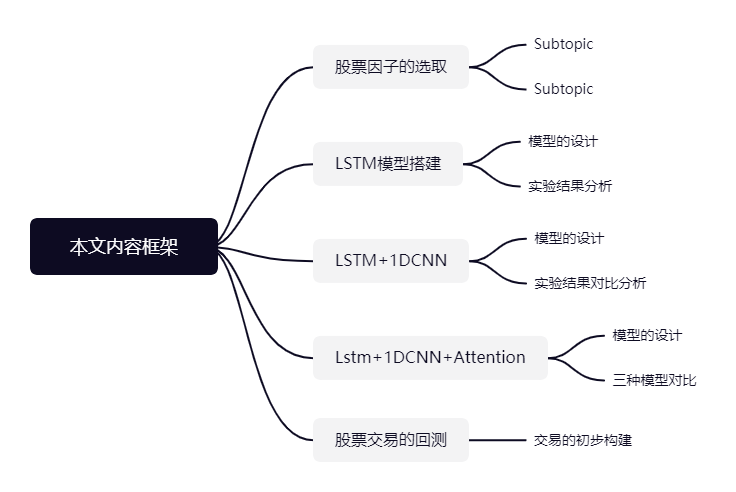
\includegraphics[width=9cm]{content summary}}
%\vspace*{-10pt}
%\end{tbox}
%\vspace*{-15pt}
\end{abstract}
% Note that keywords are not normally used for peerreview papers.
\begin{IEEEkeywords}
LSTM, 1DCNN, Attention, Keras, tensorflow, Ta-lib, BT
\end{IEEEkeywords}






% For peer review papers, you can put extra information on the cover
% page as needed:
% \ifCLASSOPTIONpeerreview
% \begin{center} \bfseries EDICS Category: 3-BBND \end{center}
% \fi
%
% For peerreview papers, this IEEEtran command inserts a page break and
% creates the second title. It will be ignored for other modes.
\IEEEpeerreviewmaketitle 
%\input{Done}
\section{股票因子的选取}\label{sec:1}


\begin{Verbatim}[breaklines=true]
引言:下面主要分享股票因子的选取,本文以沪深300成分股作为研究对象,利用akshare程序包获取了2015年6月到2022年9月的股票数据,利用Ta-lib程序包计算出与股票市场变动有很强相关性的常用指标技术指标。此内容不仅作为分享,也作为这次项目的学习记录。
\end{Verbatim}

股票量化分析分为基本面分析与技术分析两种,基本面分析又称基本分析,是以证券的内在价值为依据,着重于对影响证券价格及其走势的各项因素的分析,以此决定投资购买何种证券及何时购买。技术分析法是通过市场行为本身的分析来预测市场价格的变化方向,即主要是证券的日常交易状态,包括价格变动、交易量与持仓量的变化等资料,按照时间顺序绘制成图形或图表,或形成一定的指标系统,然后针对这些图形、图表或指标系统进行分析研究,以预测证券价格走势的方法。用技术指标对股价进行预测时,认为技术分析可以获取超额收益,做出了如下假设:股票的价格未充分反映过去的交易量与价格信息,我们称之为\underline{无效市场或者称为未达到弱有效市场}。

\smallskip


\begin{figure}[h]
     \centering
     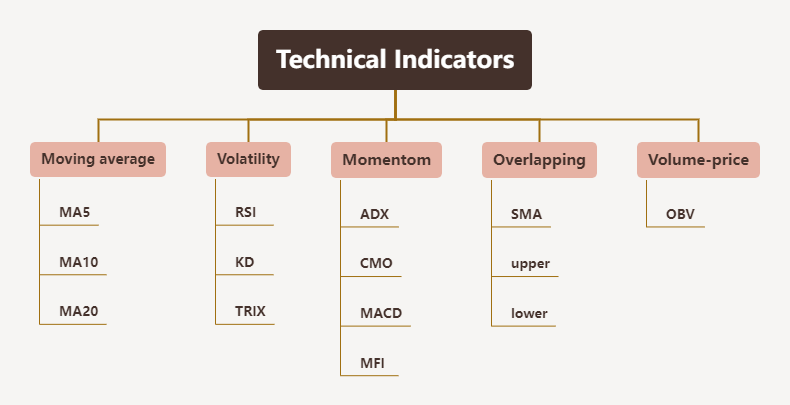
\includegraphics[width=9cm]{Stock Indictior}
     \caption{技术指标汇总}
     \label{fig:pic1}
 \end{figure}

众所周知,模型选用的因子对模型预测准确性、被解释变量的被解释程度具有密切关联,此模型根据文献\cite{任君2019基于},选了五种技术指标以及五种基本股价指标作为股票预测因子,分别为动量指标、移动均线指标、量价指标、波动率指标、重叠研究指标。技术指标的分类以及具体计算方法见\href{https://www.akshare.xyz/}{\sffamily Akshare技术文档}。


\section{LSTM模型搭建}\label{sec:2}

\subsection{长短期记忆神经网络}\label{sub:2.a}

虽然循环神经网络的目的是学习长期的依赖性,但理论的和经验的证据表明很难学习并长期保存信息,长期依赖性成了需要解决的问题。九十年代中期,德国学者Sepp Hochreiter和Juergen Schmidhuber\footnote{两位德国学者在LSTM论文中引入了CEC单元,解决了BPTT带来的梯度消失和梯度爆炸问题,被称为递归神经网络之父}提出这种循环网络的变体,带有所谓长短期记忆单元,或称LSTM,同时LSTM\cite{lstmreview,LSTM-CRF}还能解决损失函数梯度消失的问题。带有长短期记忆单元类似累加器和门控神经元:它在下一个时间步长将拥有一个权值并联接到自身,拷贝自身状态的真实值和累积的外部信号,但这种自联接是由另一个单元学习并决定何时清除记忆内容的乘法门控制的。\cite{柏万宽rnn}

遗忘门:遗忘门是以上一单元的输出$h_{(t-1)}$和本单元的输入$x_(t)$作为输入的sigmoid函数,为$C_{(t-1)}$中的每一项产生一个[0,1]内的值,来控制上一单元被遗忘的程度。

\begin{equation}
\label{eq1}
f_{(t)}=\delta(w_f[h_{(t-1)},x_{(t)}]+b_f)
\end{equation}

输入门:输入门和一个tanh函数配合控制有哪些新信息被加入。tanh函数产生一个新的候选向量$\tilde{C_t}$,输入门$\tilde{C_t}$的每一项产生一个在[0,1]内的值,控制新信息被加入的数量。
\setlength{\arraycolsep}{0.0em}
\begin{eqnarray}
i_{(t)}=\delta(w_i[h_{(t-1)},x_{(t)}]+b_i) \\
\tilde{C_t}=\delta(w_c[h_{(t-1)},x_{(t)}]+b_c) \\
C_t=i_{(t)}*\tilde{C_t}+f_(t)*C_{(t-1)}
\end{eqnarray}
\setlength{\arraycolsep}{5pt}
输出门:输出门用来控制当前的单元状态有多少被过滤掉。先将单元状态激活,输出门为其中每一项产生一个在[0,1]内的值,控制单元状态被过滤的程度决定什么样的信息要输出。
\setlength{\arraycolsep}{0.0em}
\begin{eqnarray}
o_{(t)}=\delta(w_o[h_{(t-1)},x_{(t)}]+b_o) \\
h_{(t)}=o_{(t)}*tanh(C_{(t)})
\end{eqnarray}
\setlength{\arraycolsep}{5pt}

\subsection{LSTM模型结构}

LSTM模型结构主要由LSTM层,dropout层,和dense层构成,用keras.layers的API进行模型的构建,由于计算机的计算能力有限,只用了三层LSTM,没有对层数进行比较分析。将模型的所有参数存入json文本中,方便对模型进行调参以及之后加入CNN层和Attention层。模型加入了early stopping的机制,当预测效果没有显著提升后,将终止epoch循环,为防止模型开始过拟合从而失去泛化能力。

输入特征的维数为20,用前85\%的数据作为训练集。Lstm选取时间步长为19。模型采用了滑动窗口法,滑动窗口法\cite{任君}是利用一个窗口里的所有数据来预测下一个时间点的被预测值。对窗口大小从5-20进行参数对比,也就是从一周的交易日到一个月的交易日进行搜索对比,最后选取了19作为窗口大小。
需要注意的是,前两层的lstm中的return是隐藏状态的所有值,是序列形式,而最后一层lstm只返回时间步长中最后一个输出值,也就是隐藏状态中最后一个值。
\begin{figure}[h]
     \centering
     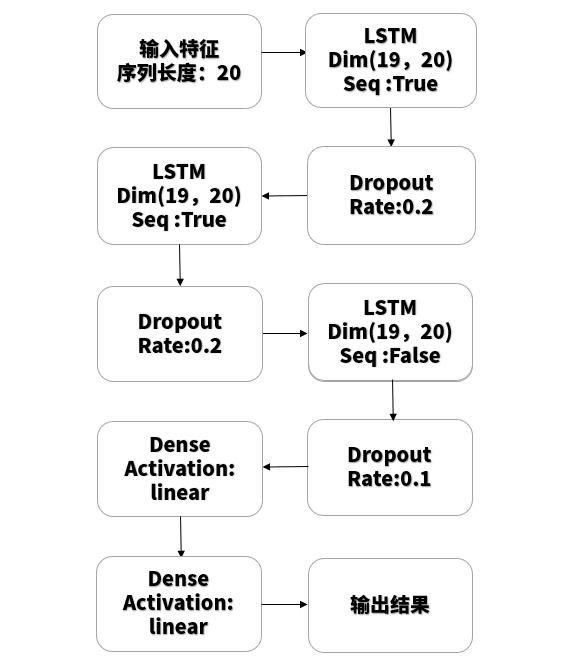
\includegraphics[width=9cm]{Model1}
     \caption{LSTM结构图}
     \label{fig:pic2}
\end{figure}

由于股票的走势不尽相同,所以本次策略欲对沪深300跑出不同模型,选取正确率大于直观预测(50\%)的股票作为回测的股票池,以下展示预测准确率等结果,均以600048为例。
\begin{figure}[h]
     \centering
     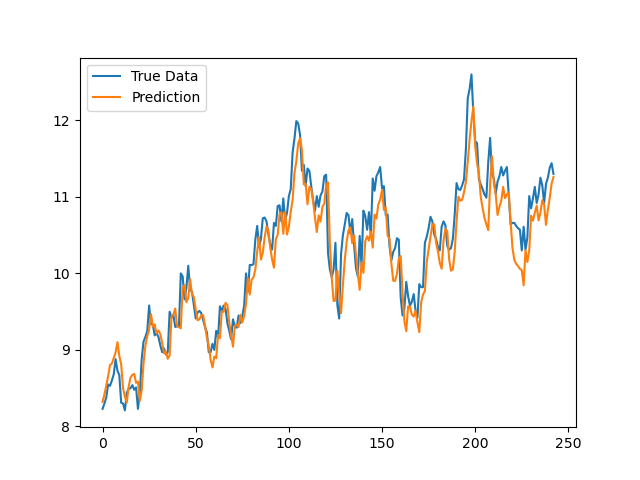
\includegraphics[width=9cm]{LSTM+CNN+ATTENTION}
     \caption{LSTM模型预测}
     \label{fig:pic3}
\end{figure}

\section{CNN+LSTM模型}

\subsection{一维卷积神经网络}

一维卷积神经网络\cite{卷积神经网络研究综述,王莉静,王宇轩}通常用于对时间序列等进行处理,其网络结构与二维卷积神经网络类似,输入序列首先经过卷积层,然后经过池化层,最后通过全连接层。二维卷积神经网络是采用一个二维矩阵的卷积核对图像的像素特征进行提取,类似地,一维卷积神经网络是采用一个一维的小序列在时间序列上滑动,从而对整个时间序列的特征进行提。
取
下图展示了一维卷积神经网络卷积计算的过程,图中的三色线分别代表着大小为3的卷积核的元素值。与二维卷积的计算过程相比,一维卷积在序列横向滑动的卷积计算过程只有横向移动。

\begin{figure}[h]
     \centering
     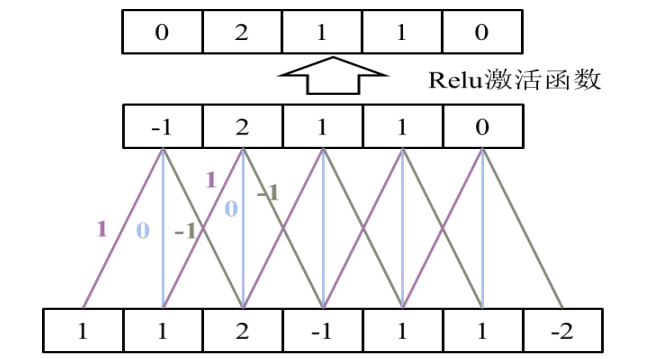
\includegraphics[width=9cm]{1dcnn}
     \caption{一维卷积核计算示意图}
     \label{fig:pic4}
\end{figure}

\subsection{LSTM+CNN模型结构}

在LSTM层之前加入keras.layers中的Conv1D,卷积核个数为50,padding=same,即不改变输入层尺寸,输入的尺寸为(19,20),以便于之后连接LSTM层。Conv1D层之后加入池化层,使用最大池化方法。加入了CNN层后,会发现模型的预测效果变差,但同时泛化能力变强,一定程度上可以改善LSTM模型的特征提取能力弱、具有表示瓶颈以及特征识别能力弱的问题,得到一个更为准确的股价指数预测模型。

\begin{figure}[h]
     \centering
     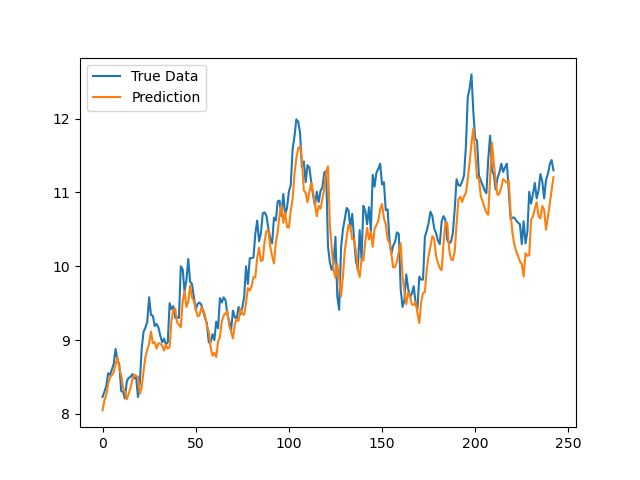
\includegraphics[width=9cm]{LSTM+CNN}
     \caption{LSTM+CNN模型预测}
     \label{fig:pic5}
\end{figure}

\section{CNN+LSTM+ATTENTION模型}

\subsection{注意力机制}

人的眼睛往往会首先注意到物体最重要的特征,并依赖这些重要特征进行物体的识别,研究者从这一现象中得到灵感,提出了注意力机制\cite{注意力机制综述}(Attention Mechanism,AM)。注意力机制可以通过对重要的信息赋予较高的权重,提高信息的利用程度,因此具有更高的可扩展性和鲁棒性\cite{seq2seq}。它克服了传统神经网络中的一些局限,如随着输入长度增加系统的性能下降、输入顺序不合理导致系统的计算效率低下、系统缺乏对特征的提取和强化等。

注意力机制从一开始就因其独特的思想深受广泛学者的喜爱,通过实验研究将其进行拓展应用于多种情景。注意力机制与传统算法的简单结合就可以提高系统的性能,因此注意力机制的提出对深度学习许多结构都有着性能提高的作用。而在2017年,Vaswani提出了Transformer模型\cite{transformer},更是将注意力机制推向了诸多应用方向的热潮。
\begin{figure}[h]
     \centering
     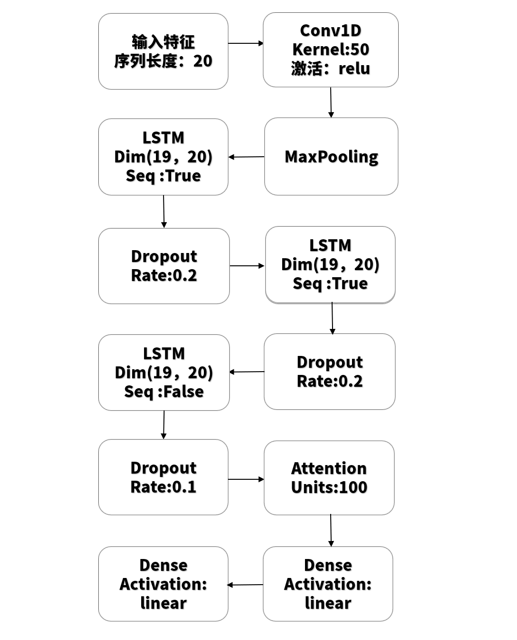
\includegraphics[width=9cm]{Model2}
     \caption{LSTM+CNN+ATTENTION结构图}
     \label{fig:pic6}
\end{figure}

\subsection{模型对比分析}
为了可以精确地比较本章所建模型之间的回归预测能力,根需要选取一些客观且能反映模型预测性能优劣的指标\cite{cnn+rlstm+att},从而使得模型之间具有可比性。本章选取了四个指标来评价所提模型以及对照模型的回归预测能力,分别是平均绝对误差、均方根误差、平均绝对百分误差以及涨跌准确率。前三个指标是用来评价模型回归预测结果与真实值的差别,而最后一个指标是用来衡量模型在回归预测过程中捕捉股票价格指数收盘价走势的能力。

\subsubsection{平均绝对误差}
平均绝对误差(Mean Absolute Error,MAE),用以计算预测值与真实值的误差绝对值的平均值,其公式如下:
\begin{equation}
\label{eq2}
MAE=\frac{1}{n}\sum_{k=1}^n|(predict_k-actual_k)|
\end{equation}
其中,predict\_k为第k个预测值,actual\_k为第k个预测值对应的真实值。MAE值可以衡量预测值与真实值的差距,MAE值越大,模型预测结果越偏离真实值。

\subsubsection{均方误差}
\begin{equation}
\label{eq3}
MSE=\frac{1}{n}\sum_{k=1}^n(predict_k-actual_k)^2
\end{equation}

\subsubsection{平均绝对百分误差}
\begin{equation}
\label{eq4}
MAPE=\frac{100\%}{n}\sum_{k=1}^n|\frac{predict_k-actual_k}{actual_k}|
\end{equation}
MAPE指标在一定程度上消除了量纲的影响,其可以用于比较模型预测不同股票时的性能。MAPE指标也是一个负向指标,其值越小说明模型的预测性能越好。

\subsubsection{预测准确率}
\begin{equation}
\label{eq5}
ACC=\frac{1}{n}\sum_{k=1}^{n}I(predict_k=actual_k)
\end{equation}
其中I为指示函数,predict\_k=actual\_k代表预测涨跌和实际涨跌相同。ACC可以描述模型捕捉涨跌信号的能力,ACC越大,模型捕捉涨跌信号能力越强,模型越优秀。

对于传统LSTM模型,LSTM+CNN模型以及LSTM+CNN+ATTENTION\cite{cnn+rlstm+att,李晨阳}模型,我们使用沪深300中的成分股600048进行演示对比。根据图3,图5,图7对比我们可以发现,传统LSTM模型捕捉涨跌信号的能力与加入CNN接近,但是均低于LSTM+CNN+ATTENTION模型,再加入注意力机制之前,会发现CNN模型的引入反而将模型的预测精度降低,这可能是CNN提供的特征模型无法很好分析。

\begin{figure}[h]
     \centering
     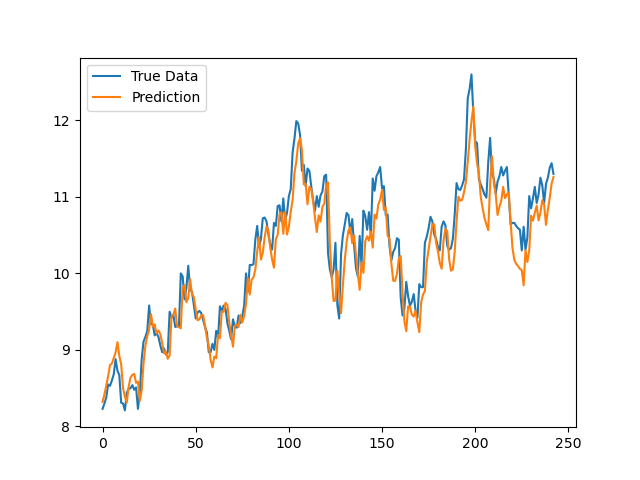
\includegraphics[width=9cm]{LSTM+CNN+ATTENTION}
     \caption{LSTM+CNN+ATTENTION模型预测}
     \label{fig:pic7}
\end{figure}

由表格1可知,加入了注意力机制后,可以发现模型不管从拟合的精度还是涨跌准确率都优于其他两个模型,LSTM+CNN+ATT模型的MSE在LSTM模型的基础上降低了40\%左右,这说明加入了CNN以及注意力机制之后,能实质性地改进模型的预测能力。所以我们得到的结论是,最好的模型是LSTM+CNN+ATT模型,次优的是LSTM模型,表现最差的是CNN+LSTM模型。

\begin{table}[!t]
	\centering
	\caption{Tree different model comparison}
	\label{tab:math-space}
	\begin{IEEEeqnarraybox}[\IEEEeqnarraystrutmode\IEEEeqnarraystrutsizeadd{2pt}{1pt}]{v/c/v/r/v/c/v/c/v/c/v}
		\IEEEeqnarrayrulerow\\
		& \mbox{{\bf Model}} && \mbox{{\bf MAE}} && \mbox{{\bf MSE}} &&
		\mbox{{\bf MAPE(\%)}} && \mbox{{\bf ACC(\%)}} &\\
		\IEEEeqnarraydblrulerow\\
		\IEEEeqnarrayseprow[3pt]\\
		& \mbox{LSTM} && \mbox{0.2805} && \mbox{0.1305} && \mbox{2.673} && \mbox{0.5165}&\IEEEeqnarraystrutsize{0pt}{0pt}\\
		\IEEEeqnarrayseprow[3pt]\\
		\IEEEeqnarrayrulerow\\
		\IEEEeqnarrayseprow[3pt]\\
		& \mbox{LSTM+CNN} && \mbox{0.3257} && \mbox{0.1658} && \mbox{3.1172} && \mbox{0.5023} &\IEEEeqnarraystrutsize{0pt}{0pt}\\
		\IEEEeqnarrayseprow[3pt]\\
		\IEEEeqnarrayrulerow\\
		\IEEEeqnarrayseprow[3pt]\\
		& \mbox{LSTM+CNN+ATT} && \mbox{0.215} && \mbox{0.0815} && \mbox{2.0838}&&\mbox{0.5413} &\IEEEeqnarraystrutsize{0pt}{0pt}\\
		\IEEEeqnarrayseprow[3pt]\\
		\IEEEeqnarrayrulerow
	\end{IEEEeqnarraybox}
\end{table}

\section{股票交易的回测}

\subsection{模型回测}

回测(Back Test)是根据历史数据来验证交易策略的可行性和有效性的过程。做回测是希望可以用回测后的表现来评估未来实盘表现。我们假设如果回测结果好,实盘结果也不会太差,也就是说我们假设回测时的市场历史表现会在未来重演。现在提供回测的策略平台有很多,比如国泰安,BigQuant,掘金量化等,但是根据策略的不同,假设的不同,或者股票指数的不同,回测的逻辑结构也不尽相同,如果没有能力搭建自己的回测算法,那说明还没有进入股票量化门槛。

本文根据以上对股票时间序列的预测模型,搭建了结合止盈止损策略的较为浅显回测算法,由于是第一次做股票量化,所以此算法只能提供部分验证性。回测结果的好坏可以很大程度反应运用该模型的历史收益率,是在进行了较多的理想假设的基础上实现的:

\begin{enumerate}[label=hypothesis]
    \item 忽略操作员的交易时需要的时间以及失误
    \item 操作员或者策略者是完全理性的,是策略至上主义者
    \item 认为数据都是可以及时得到的,也有充足的时间训练模型
    \item 模型对股票的适用性在短时间内不发生变化
\end{enumerate}

\subsection{回测算法的搭建}

本文采用较为简单的固定止损(需要金融学知识较少),每次进场都带有固定点数的止损进场,而固定的点数也是根据自己策略的级别和资金的规模决定的,止盈也是如此,虽然看起来有些机械化但是至少能够保护账户的安全。该模型的止损率设置为-0.05(非常保守),止盈率设置为0.10,初始资金为500,000元,股票最大持有天数为5天,即一周的交易日,这也是短线策略较常用的参数。

回测算法包括两大模块,分别为Create\_Pool和Account,Create\_Pool的功能是load那些事先训练好的进入初始股票池的模型,根据预测下一天的股票价格计算预测当天收益率,筛选出预测收益率为正的股票并根据收益率排序作为第二天的股票池。Account模块是对个人账户的模拟,会根据止盈止损策略进行股票买卖,并进行必要信息的记录。以下以沪深300中的30支成分股作为初始股票池,对于2022年11月中的交易日进行回测。

\begin{figure}[h]
     \centering
     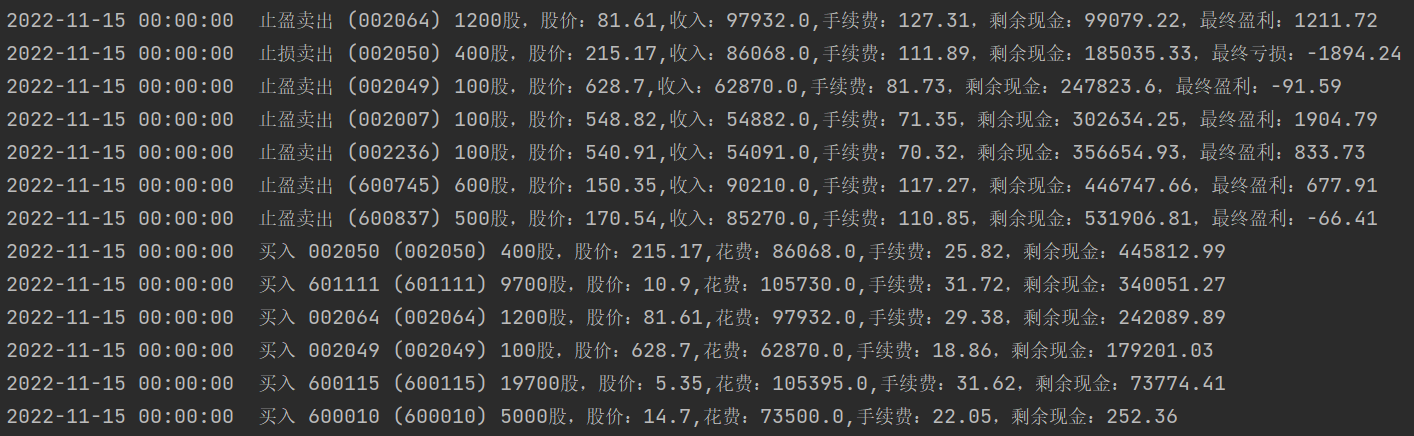
\includegraphics[width=9cm]{trade}
     \caption{11-15的交易详情}
     \label{fig:pic8}
\end{figure}


\begin{figure}[h]
     \centering
     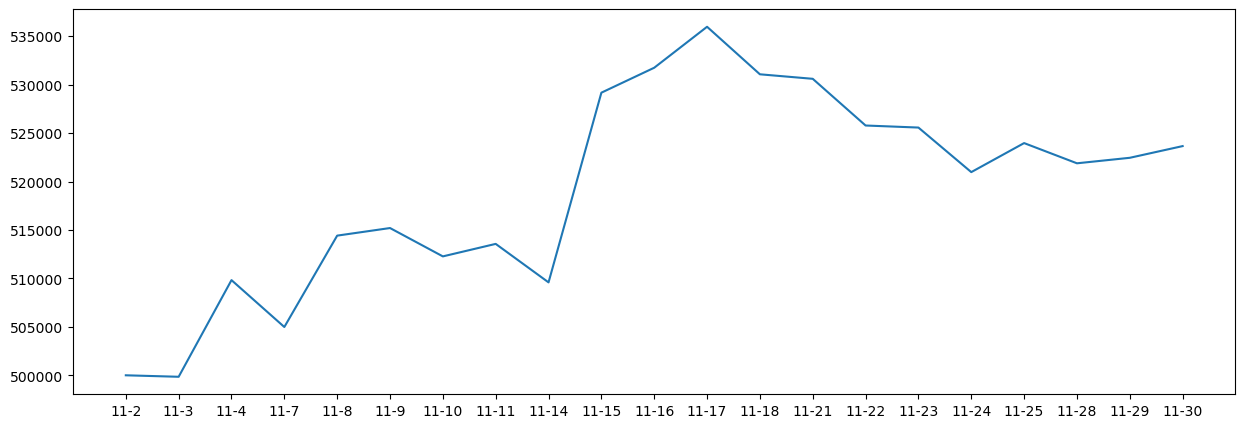
\includegraphics[width=9cm]{moneychange}
     \caption{11月模型回测总资金情况}
     \label{fig:pic9}
\end{figure}

由图9可知,模型在11月内一月的收益达到了23658元,说明模型在股市中获利的能力是非常不错的,但是也可以发现的问题是,模型的表现随着时间的推移逐渐下降,到17号之后开始收益率为负了。这是因为由于计算机算力限制,我们用的模型是不随着时间更新的,由于股市的波动是非常大的,再加上模型预测n天后的误差不是线性上升而是指数上升。这为后续的研究提供了思路,可以制作随着时间不断更新的策略模型,编写更有效率的代码来改进该策略。


\section*{致谢}\label{a:g}

本文不仅是一份项目汇报,更是一份学习的记录,感谢谢传龙和童行伟两位教授的教学与指导,没有他们为学生制定的学习计划,作者不可能开始去接触金融量化,并产生了极大的学习兴趣。同时需要感谢keras-team\href{https://github.com/keras-team/keras/projects/1}{(git)},唐宇迪博士\href{https://github.com/PlayPurEo/ML-and-DL/tree/master/pytorch}{(git)},Gambler\_Evolution\href{https://github.com/wbbhcb/stock_market/blob/master}{(git)}这些开发者在github上提供了开源学习代码,为此次项目提供了许多的借鉴意义和学习支持。最后要感谢IEEE\footnote{电气和电子工程师协会(IEEE,全称Institute of Electrical and Electronics Engineers)是一个美国的电子技术与信息科学工程师的协会,是目前世界上最大的非营利性专业技术学会,其会员人数超过40万人,遍布160多个国家。}提供的Latex模板,为编写论文提供了"方便"。

\IEEEtriggeratref{25}
\bibliographystyle{IEEEtran}
\bibliography{ABIB}


\end{document}